%\lipsum[4-4]
In this chapter there are presented the future steps in research on outliers detection on railways WSN-based smart grid.


%%%%%%%%%%%%%%%%%%%%%
%%   Smart metering Systems
%%%%%%%%%%%%%%%%%%%%%
\section{Evaluation of effect of undetected outliers in railway WSN}


During the state of the art, the definition of "what is an outlier in railways WSN" was slightly covered, resulting in raising the research question:
	
	
\vspace{0.5em}
{\centering{
		\framebox[\linewidth]{
	\textbf{What is the effect of an undetected outlier in an railways WSN?}
} }}\par
\vspace{1.5em}

A railways WSN is focused on acquiring the data (in forms of measurements) from the railways environment with the purpose of providing that information to a subsystem (such as a decision support system). Having this in mind, an assumption should be made to define the outlier as the effect of erroneous information retrieved from the DSS due to erroneous data from the measurement. A major contribution of an outlier detection mechanism is the validation of the quality of the output of the DSS. In particular, if a measurement or a set of measurements are detected as outliers, the DSS will have the information of the quality of his output, as is shown in figure \ref{fig:evaluation}.

\begin{figure}[h!]
	\centering
	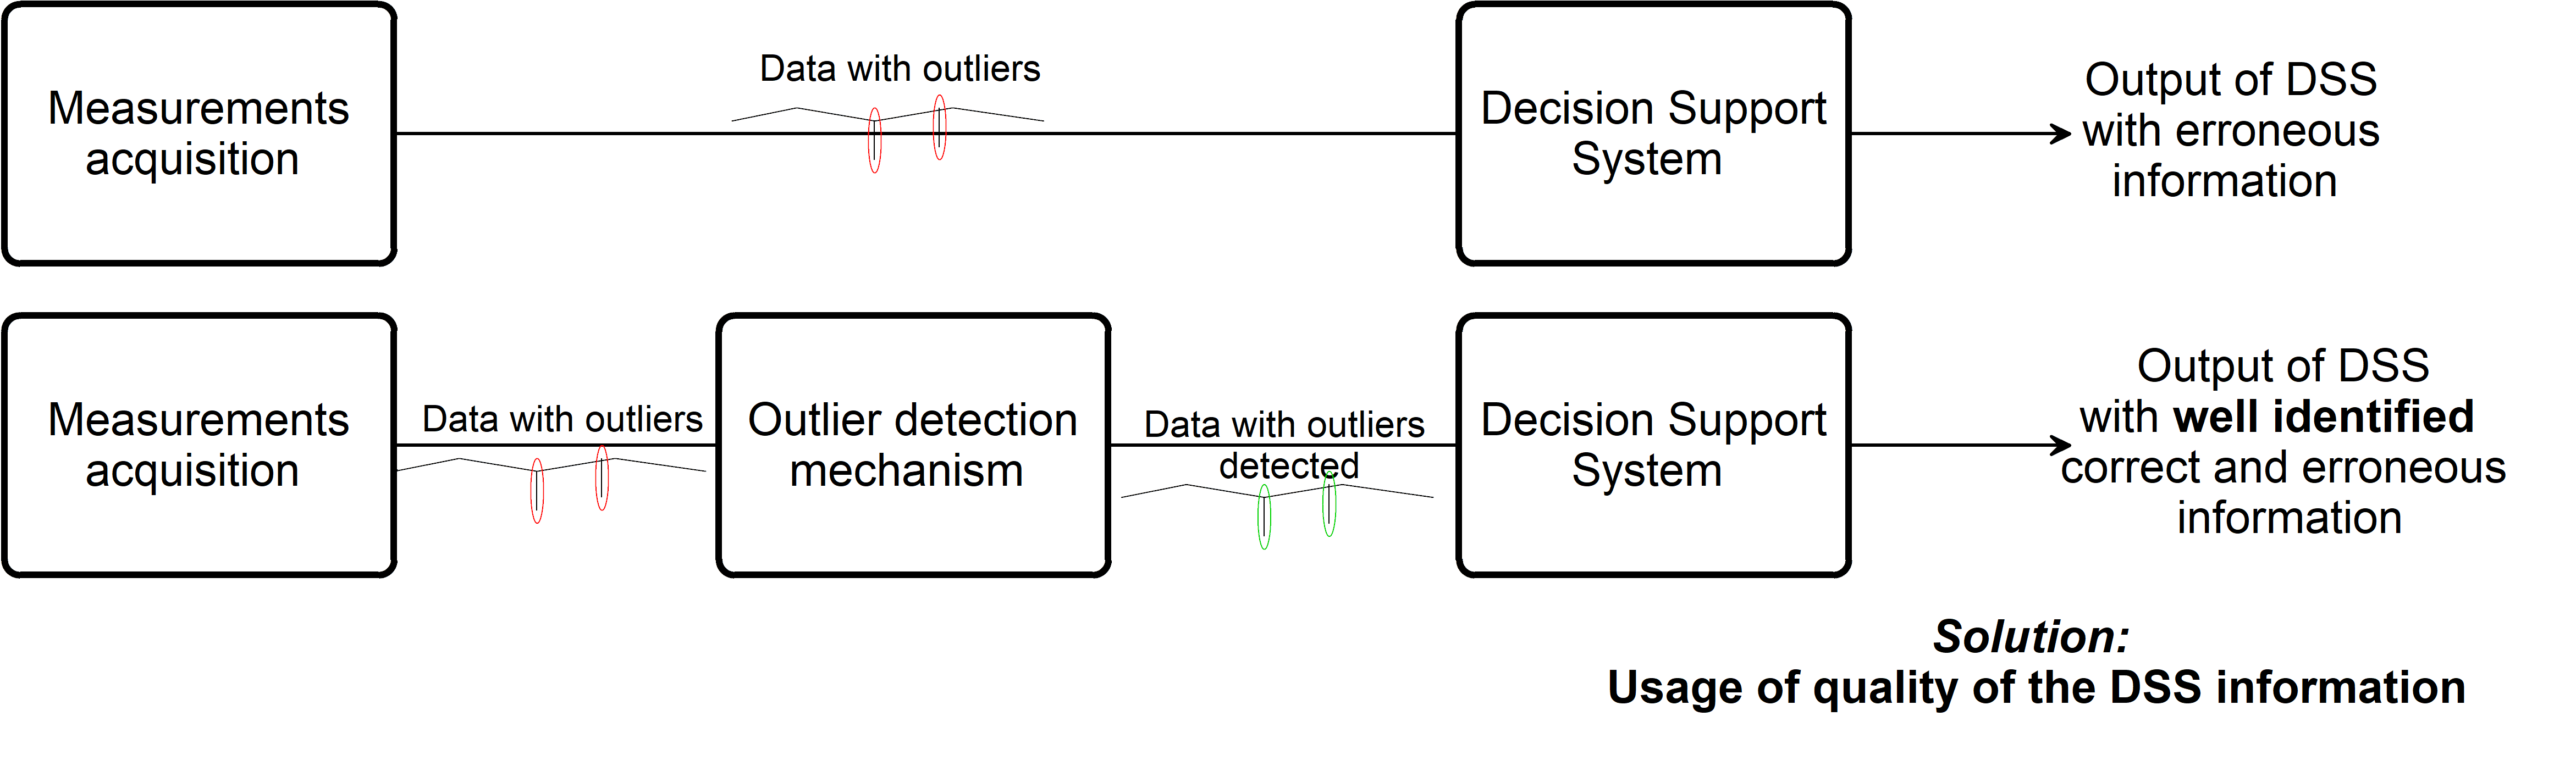
\includegraphics[width=1.03\textwidth,keepaspectratio]{figures/evaluation}
	\caption{Comparison of the output of DSS with and without an outlier detection mechanism. }
	\label{fig:evaluation}
\end{figure}

It is important at this moment to present examples of DSS. Eco-driving strategies and timetable planning require conservative measurements of energy consumption in several points of the railway electrical system, where the situations of outliers should result, in example, in default outputs of DSS; On other side, preventive maintenance may find resourceful the presence of outliers considering that those outliers reflect anomalous behavior due to unknown external effects (on the measurement).

The methodology will embrace the simulation of the railway WSN system. With a well defined simulation model that mimics the behavior of the DSS, the measurements acquisition system and the wireless network, the effect of undetected outlier can be evaluated before and after the DSS.

Considering the literature, two possibilities will be considered as a starting point for this railway WSN system simulator: the NS-3 and the contiki-cooja network simulators. However, for the future research, a higher analysis on the available simulators must be considered.


\section{Selection of Outlier detection mechanism}

On the previous section, the need of a simulation model was presented. However, based on real data from railway systems (or similar) can validate the implementation of an outlier detection mechanism.

In this way, a set of outlier detection mechanisms can be validated with a given test-bench. The research question that can be raised is the following:

\vspace{0.5em}
{\centering{
		\framebox[\linewidth]{
			\textbf{How to effectively detect an outlier in a railways WSN?}
} }}\par
\vspace{1.5em}

One main requirement of the energy consumption evaluation in a railway environment is the need to acquire AC measurements and extract, at the node, the RMS continuous values. Despite the continuous values are expected to be sent to a data concentrator at a periodic timestamp (much lower than the 50Hz/16,6Hz of the railways grid) the acquisition system must be constantly acquiring the variables and making the computational needed calculations to have an effective energy measurement. Therefore, the computational needs for such system should be considerable. In addition, it is expected that such sensors have enough computational resources to implement certain outlier detection mechanisms that require extensive computational efforts.

This way, the computational requirements should not be considered in a initial approach, in the perspective of the node energy consumption. Complementarity, the literature has supported the usage of on-line outlier detection techniques that increases the computational effort towards the reduction of transmission energy consumption (avoiding the transmission of erroneous data).

The methodology expected to answer the raised research question is, at a first instance, a combination of the \cite{class:xu:2012} methodology (by using a KNN-SVM technique) and the \cite{nn:abid:2016} methodology (that focuses the evaluation of the data values of a given time-slot by using a $k^{th}-nn$ procedure).

A first test-bench would be the data returned by a monitoring system developed in DEEC. In the figure \ref{fig:website} is presented the data that is monitoring a wind generator power converter.
\begin{figure}[h!]
	\centering
	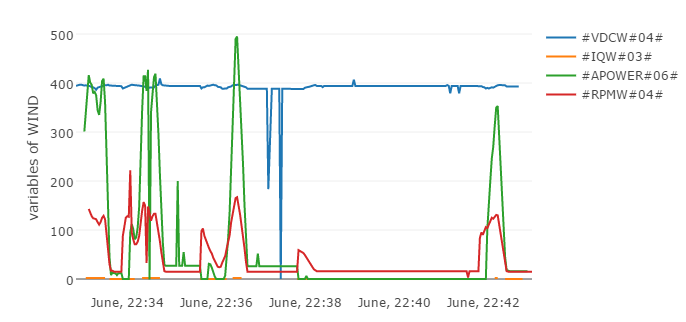
\includegraphics[width=0.90\textwidth,keepaspectratio]{figures/website}
	\caption{Website representation of ten minute log of wind generator variables. }
	\label{fig:website}
\end{figure}

The wind generator in question is designed to achieve 2kW at nominal power. However, the low and inconstant wind speed conditions are the cause of the viewed spikes in the power (green line) and in the rotor velocity (red line).

A major contribution of an oultier detection mechanism will be the pre-processing of the data before is transfered to the data-concentrator. An important note should be taken since this is a wired test-bench and the data is collected from the power converted with the spikes, showed in upper graph of figure \ref{fig:wind_power}, and then sent to the data concentrator.

\begin{figure}[h!]
	\centering
	\includegraphics[width=1\textwidth,keepaspectratio]{figures/wind_power}
	\caption{Data log of four days of wind generator variables. }
	\label{fig:wind_power}
\end{figure}

With the knowledge of the behavior of the wind turbine, it is known that the maximum power will not be greater than, at most 200\% of the nominal power. An interesting outlier detection technique in this application will be a technique that does not require the apriori knowledge of the measurements. In the bottom graph is presented the graph that removes the erroneous data (based only on the knowledge that the power should be lower than 4kW).


